\section{Introduction}
This chapter will outline the usage of Bre\'guet's range equations in two methods for finding the pareto frontier of optimal range and endurance tradeoffs for an aircraft, given certain parameters. Additionally, a method for determining a tradeoff frontier for endurance of an aircraft's flight and the radius of its loiter. Lastly, the application of this approach will be explained in detail.\par
\section{Current Methodology}
\section{Deriving Bre\'guet Equations}
Two main equations are derived from the general range equation seen in Eq. \ref{eqRangeEq}. The first logically flows from the need to maximize range while assuming a constant thrust specific fuel consumption (constant altitude and throttle setting). Maximizing $V/T_A$ will maximize range and $T \approx T_R = D$ where $D$ is drag. Thus, to maximize range, the aircraft must be flown at $(D/V)_{min}$. The following equivalent equations follow from the assumption that the aircraft will fly at straight, level, unaccelerated flight.
\begin{align}
    T_A&=D = C_Dq_{\infty}S \dfrac{W}{L} = \dfrac{C_Dq_{\infty}S(W)}{C_Lq_{\infty}S} = \dfrac{C_D}{C_L}W\\
    L &= W = C_Lq_{\infty}S = C_L\dfrac{1}{2}\rho_{\infty}V^2_{\infty}S \Rightarrow V_{\infty} = \sqrt{\dfrac{2W}{\rho_{\infty}C_LS}}
    \label{eq: VequivalentEq}
\end{align}
These equations can be used in the general range equation shown in Eq. \ref{eq:genRangeFull}.
\begin{equation}
\label{eq:genRangeFull}
    \begin{aligned}
        R &= \int_{W_f}^{W_i}\sqrt{\dfrac{2W}{\rho_{\infty}C_LS}}\left(\dfrac{1}{TSFC}\right)\left(\dfrac{C_L}{C_D}\right)\left(\dfrac{1}{W}\right)dW\\
        R &= \int_{W_f}^{W_i}\sqrt{\dfrac{2W}{\rho_{\infty}S}}\left(\dfrac{1}{TSFC}\right)\left(\dfrac{C_L^{1/2}}{C_D}\right)\left(\dfrac{1}{W}\right)dW\\
    \end{aligned}
\end{equation}
Further simplifying assumptions are used in general aircraft performance in \cite{IntroACMechanics} to derive the following Bre\'guet range equation in Eq. \ref{eq:LinRangeEq}. These include a constant altitude which implies a constant density, $\rho_{\infty}$, a constant angle of attack which makes $C_L$ and $C_D$ constant, and similar to the general equation, TSFC is constant.
\begin{equation}
\label{eq:LinRangeEq}
    \begin{aligned}
        R &= \sqrt{\dfrac{2}{\rho_{\infty}S}}\left(\dfrac{1}{TSFC}\right)\left(\dfrac{C_L^{1/2}}{C_D}\right)\int_{W_f}^{W_i}\dfrac{dW}{\sqrt{W}}\\
        R &= \sqrt{\dfrac{2}{\rho_{\infty}S}}\left(\dfrac{2}{TSFC}\right)\left(\dfrac{C_L^{1/2}}{C_D}\right)(\sqrt{W_i}-\sqrt{W_f})
    \end{aligned}
\end{equation} \par
In addition to the linear range equation, another simplification of the general range equation involves assuming constant cruise velocity, a constant angle of attack, and a constant thrust specific fuel consumption. This equation is referred to in \cite{IntroACMechanics} as the constant speed cruise range equation. Using the general range equation in \ref{eq:genRangeFull} and substituting $V$ in for the equivalent formula presented in \ref{eq: VequivalentEq}, the following equation is derived.
\begin{equation}
    R = \dfrac{V}{TSFC}\left(\dfrac{C_L}{C_D}\right)\ln{\dfrac{W_i}{W_f}}
    \label{eq: NLRange}
\end{equation}
This equation is maximized when $V\dfrac{C_L}{C_D}$ is maximized or equivalently when $\dfrac{C_L^{1/2}}{C_D}$ is maximized.

\section{Flight Mapping}
Parameters for the flight plan can either be user-defined or be defined to maximize performance for a best case scenario. In the interest of simplicity, the T-37 will be used as a general example for how parameters are extracted for maximizing performance and the F-15C will be used to identify parameters from the existing NASIC model. \par
The theoretical drag polar for an aircraft is shown in Eq. \ref{eq: dragpolar}.
\begin{equation}
    C_D = C_{D_0} + kC_L^2
    \label{eq: dragpolar}
\end{equation}
where $C_{D_0}$ is the parasitic drag coefficient and $k = 1/\pi A_Re$ for when $A_R$ is the aspect ratio of the aircraft and $e$ is the Oswald's efficiency factor. Yechout \cite{IntroACMechanics} introduces the T-37's drag polar equation for an example that maximizes the $C_L/C_D$ and $C_L^{1/2}/C_D$. The drag polar equation for the T-37 is shown to be  
\begin{equation*}
    C_D = 0.02 + 0.057C_L^2.
\end{equation*}
In order to maximize $C_L/C_D$ and $C_L^{1/2}/C_D$, Eq. \ref{eq:maxlift} is used to solve for $C_L$ where
\begin{equation*}
    C_{L_MR} = \sqrt{\dfrac{0.02}{3(0.057)}} = 0.342.
\end{equation*}
Using this value for $C_L$, $C_D$ can be calculated using the T-37 drag polar.
\begin{equation*}
    C_D = 0.02 + 0.057(0.342)^2 = 0.0267
\end{equation*}
As a result, flying at these values for maximizing $C_L$ and $C_D$ will maximize range and endurance \cite{IntrotoAero}. These values will allow for the use of a continuous range equation introduced in Eqs. \ref{eq:LinRangeEq} and \ref{eq: NLRange}. \par
Beginning with the formulation for the linear range equation, the intercept for maximum range and the intercept for starting fuel must be determined. Since the flight pattern will include an initial warm-up, take-off, and climb, the model assumes that the fuel burn and distance from initial starting point are given though these can also be calculated using optimal climbing conditions discussed in \cite{IntroACMechanics}. To identify the point where the aircraft starts its egress to a point of interest, the model requires the vertical value to be in terms of fuel reserve. Thus, to determine the slope of this line, the fuel burn must be converted to the fuel reserve of the aircraft. For example, assume the T-37 flies 1.5 miles on its climb to cruise and burns 900 lbs of fuel during take-off procedures and climb to cruise. Given that the take-off weight and dry weight (no fuel) of the aircraft is 6,598 lbs and 3,869 lbs respectively, the fuel reserve percentage is at 0.864. The calculations are shown more succinctly below.
\begin{equation*}
    \dfrac{\textit{take-off weight}- \textit{fuel burned}}{\textit{take-off weight}} = \dfrac{6598-900}{6598} = 0.864
\end{equation*}
The point (1.5,0.864) is the first point to determine the equation for the egress line. The next point needed will be determined by Eq. \ref{eq:LinRangeEq}. Given that the thrust specific fuel consumption (TSFC) for the T-37 at 30,000 ft is 0.000232 lbs/s, the $\rho_\infty$ is 0.001267 slug/ft$^3$ using the US Standard Atmosphere, and the span of the T-37 is 184 ft$^2$, the solution for maximum range can be found.
\begin{align*}
    R  &= \sqrt{\dfrac{2}{\rho_{\infty}S}}\left(\dfrac{2}{TSFC}\right)\left(\dfrac{C_L^{1/2}}{C_D}\right)(\sqrt{\textit{climb to cruise weight}}-\sqrt{\textit{dry weight}})\\
    &= \sqrt{\dfrac{2}{0.001267(184)}}\left(\dfrac{2}{0.000232}\right)\left(21.9\right)(\sqrt{6598-900}-\sqrt{3869})\\
    &=1391.2\textit{ miles}.
\end{align*}
Thus, the second point for the equation of the egress line is (1391.2,0).\par
The ingress equation is found in a similar fashion using the slope for the ingress line and using the user-defined fuel reserve required as the point for use in the point-slope formula. For example purposes, the fuel reserve required  for the T-37 will arbitrarily be chosen to be 20\%, making the point for the ingress equation (0.2,0).\par
To determine the slope for the egress equation, the point-slope formula is used, making the equations of the lines:
\begin{align}
    \textit{fuel remaining in egress} &= 0.865 - 0.000621(\textit{miles traveled})\\
    \textit{fuel remaining in ingress} &= 0.20 + 0.000621(\textit{miles traveled}).
\end{align}
The intercept of these lines will determine the maximum range that an aircraft can egress to a point of interest and return to base with the required fuel reserve. The vertical distance between these lines is the fuel available for loiter and/or combat time. Figure \ref{fig:exT37} shows the results of the previous calculations and plots the resulting ingress equation, egress equation, and fuel available for loiter and combat at 300 miles. The loiter and combat altitudes are variable and depend on the flight plan, but must be specified.\par
\begin{figure} 
    \centering
    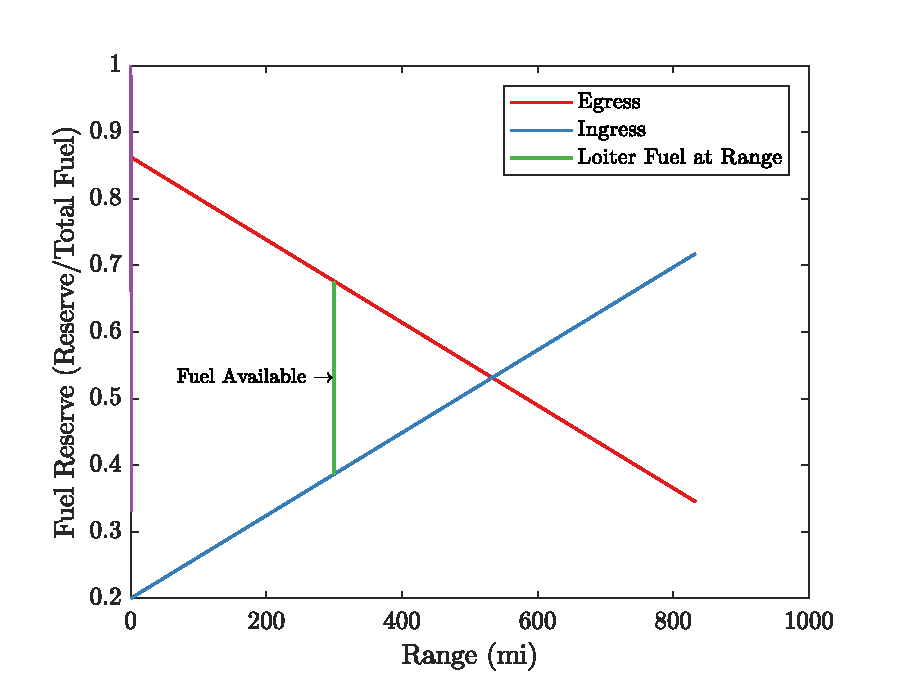
\includegraphics[width = 8cm]{Thesis/Method/ExampleFlightT37.eps}
    \caption{Example Flight Plan T-37}
    \label{fig:exT37}
\end{figure}
The non-linear equation for range is the equivalent formula presented in \ref{eq: NLRange}. The only additional parameter needed to solve for maximum range in this equation is the velocity which is assumed constant at the $C_L/C_D$. This is equivalent to finding the velocity at the maximum $\dfrac{C_L^{1/2}}{C_D}$. In the example case, since the drag polars at each mach number are unknown, a velocity of 0.5 mach at sea level will be used. Solving Eq. \ref{eq: NLRange} for fuel reserve, the egress equation becomes
\begin{equation}
    \textit{fuel remaining} = \dfrac{\exp\left[\left(\dfrac{-R}{V}\right)\dfrac{(TSFC)}{C_L/C_D}\right]W_i-\textit{dry weight}}{\textit{full weight} - \textit{dry weight}}.
\end{equation}
The equation for ingress is similarly derived as 
\begin{equation}
    \textit{fuel remaining} =\dfrac{\exp\left[\left(\dfrac{R}{V}\right)\dfrac{(TSFC)}{C_L/C_D}\right]W_i-\textit{dry weight}}{\textit{full weight} - \textit{dry weight}}.
\end{equation}
In order for the equations to accurately represent fuel reserve, the given intercept must be determined for fuel burned during climb to cruise and take-off as well as the intercept for fuel reserve required.\par

% BELOW IS EXTRACTION
Parameters for the F-15C's $C_L\text{ and }C_D$ performance are referenced in Figure \ref{fig:machSpeedByGroup}. Each line in the graph represents a mach number which is formed by the value for each coefficient of lift ($C_L$) and the associated coefficient of drag ($C_D$). These are found from historical flying data for each specific aircraft. From the matrix of these values, the lift over drag and $C_L^{1/2}/C_D$ maximums can be found. Where $C_L^{1/2}/C_D$ is maximized, the respective mach number and $C_L/C_D$ can be pulled into the model as a parameter.\par
An example of drag polar outputs from the existing model are shown in Figure (PLACE) for reference. Using 

\begin{figure}%
    \centering
    \subfloat[Lift versus drag curves for all mach numbers.]{{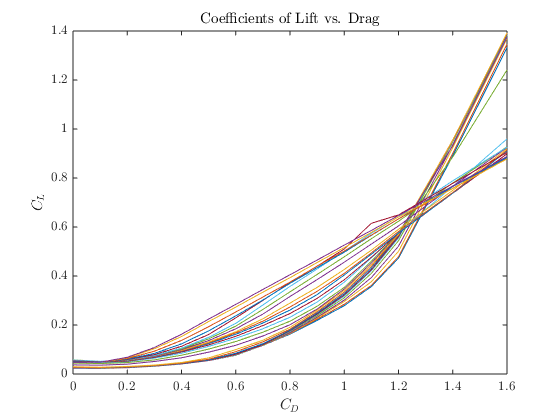
\includegraphics[width=7cm]{Thesis/Method/AllMachNumbers.png} }}%
    \qquad
    \subfloat[Lift versus drag curves defined by mach group.]{{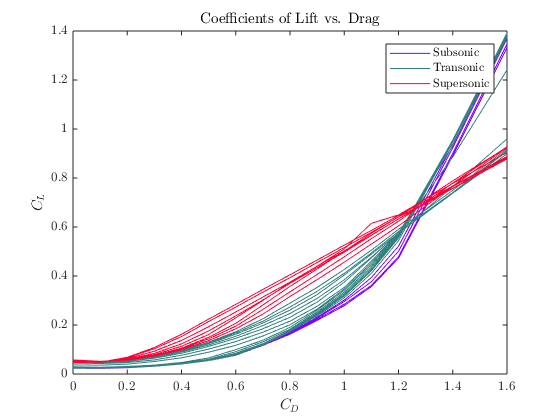
\includegraphics[width=7cm]{Thesis/Method/MachSpeedByGroup.png} }}%
    \caption{Coefficients of lift versus drag for the F-15C.}%
    \label{fig:machSpeedByGroup}%
\end{figure}


